\subsection{Detector}

The detector is a silicon photodiode (Photonic Detectors Inc.\ PDB-C108) with a
circular active area of diameter $\tfrac{1}{4}$~inch, connected to a current-to-voltage
preamplifier. The diode is operated in \textbf{photovoltaic mode} (cathode grounded)
to minimise noise.

\begin{figure}[h]
    \centering
    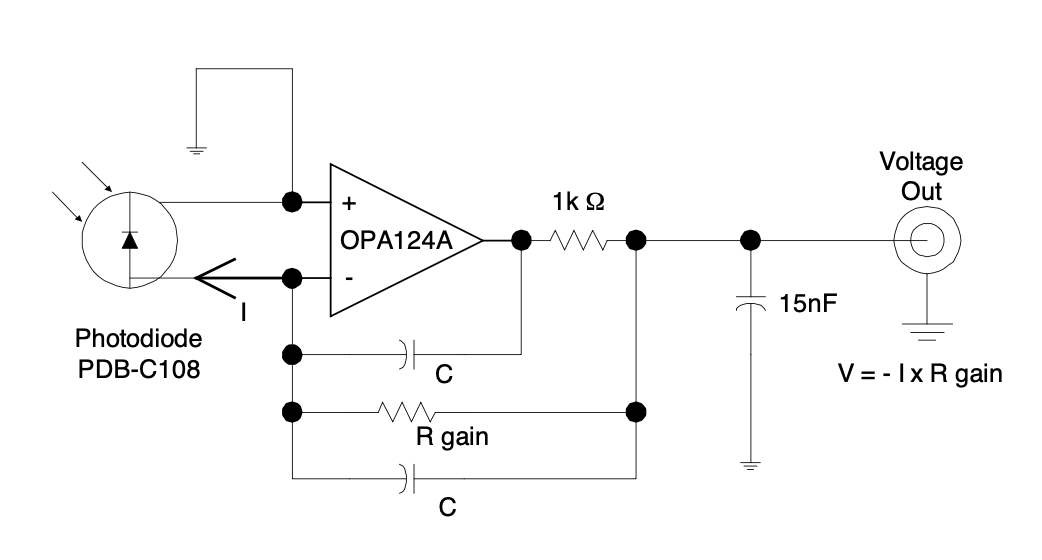
\includegraphics[width=0.55\textwidth]{figures/detector.png}
    \caption{Schematic of the photodiode preamplifier circuit.}
\end{figure}

\subsubsection*{Photodiode Response}

When light of wavelength $\lambda$ and power $P$ is incident on the photodiode, the
generated photocurrent is :
\begin{equation}
    I_{\text{ph}} = \mathcal{R}(\lambda)\cdot P
\end{equation}
where $\mathcal{R}(\lambda)$ is the spectral responsivity of the diode (A/W). The
responsivity is related to the quantum efficiency $\eta_Q$ by :
\begin{equation}
    \mathcal{R}(\lambda) = \eta_Q \cdot \frac{e\lambda}{hc}
\end{equation}
where $e$ is the electron charge, $h$ is Planck's constant, and $c$ is the speed of
light. At the operating wavelength of 795~nm, the specified responsivity is
$\mathcal{R} = 0.6$~A/W, giving a quantum efficiency of :
\begin{equation}
    \eta_Q = \mathcal{R}\cdot\frac{hc}{e\lambda}
    = 0.6 \times \frac{(6.626\times10^{-34})(3\times10^8)}
                      {(1.602\times10^{-19})(795\times10^{-9})}
    \approx 93.5\%
\end{equation}

\subsubsection*{Current-to-Voltage Conversion}

The preamplifier is a transimpedance amplifier : the photocurrent $I_{\text{ph}}$ flows
through a gain resistor $R_{\text{gain}}$, producing an output voltage :
\begin{equation}
    V_{\text{out}} = -I_{\text{ph}} \cdot R_{\text{gain}} = -\mathcal{R}P\cdot R_{\text{gain}}
\end{equation}
The negative sign reflects the inverting configuration. Substituting the lamp intensity
at 795~nm ($P = 1.7\ \mu$W) and $R_{\text{gain}} = 1\ \text{M}\Omega$ :
\begin{equation}
    V_{\text{out}} = -0.6 \times 1.7\times10^{-6} \times 1\times10^{6} = -1.02\ \text{V}
\end{equation}
The preamplifier output is maintained between $-2.0$ and $-8.0$~V to avoid saturation.
Three selectable gain resistors are available :

\begin{table}[h]
    \centering
    \begin{tabular}{ccc}
        \hline
        $R_{\text{gain}}$ & 3\,dB bandwidth & Noise (peak-to-peak) \\
        \hline
        $100\ \text{k}\Omega$ & 60.0~kHz & 3~$\mu$V \\
        $1\ \text{M}\Omega$   & 17.0~kHz & 4~$\mu$V \\
        $10\ \text{M}\Omega$  &  5.5~kHz & 8~$\mu$V \\
        \hline
    \end{tabular}
    \caption{Preamplifier gain settings and corresponding bandwidths and noise levels.}
\end{table}

\subsubsection*{Noise Analysis}

The dominant noise source in the transimpedance amplifier is the \textbf{Johnson noise}
of $R_{\text{gain}}$. The RMS noise voltage over a bandwidth $\Delta f$ is :
\begin{equation}
    V_{n,R} = \sqrt{4k_BT\,R_{\text{gain}}\,\Delta f}
\end{equation}
where $k_B$ is the Boltzmann constant and $T$ is the absolute temperature. At room
temperature ($T = 300$~K) with $R_{\text{gain}} = 10\ \text{M}\Omega$ and
$\Delta f = 1$~kHz :
\begin{equation}
    V_{n,R} = \sqrt{4\times(1.38\times10^{-23})\times300\times10^7\times10^3}
    \approx 12.9\ \mu\text{V}_{\text{rms}}
\end{equation}
The \textbf{shot noise} contribution from the photocurrent $I_{\text{ph}}$ is :
\begin{equation}
    V_{n,\text{shot}} = R_{\text{gain}}\sqrt{2eI_{\text{ph}}\,\Delta f}
\end{equation}
The total output noise is then :
\begin{equation}
    V_{n,\text{total}} = \sqrt{V_{n,R}^2 + V_{n,\text{shot}}^2}
                       = \sqrt{4k_BT R_{\text{gain}}\Delta f
                              + 2eI_{\text{ph}}R_{\text{gain}}^2\,\Delta f}
\end{equation}
The signal-to-noise ratio (SNR) is therefore :
\begin{equation}
    \text{SNR} = \frac{V_{\text{out}}}{V_{n,\text{total}}}
               = \frac{\mathcal{R}P\,R_{\text{gain}}}
                      {\sqrt{4k_BT R_{\text{gain}}\Delta f
                             + 2e\mathcal{R}P\,R_{\text{gain}}^2\,\Delta f}}
\end{equation}

\subsubsection*{Low-Pass Filter and Detector Electronics}

The preamplifier incorporates a two-pole low-pass filter with $-3$~dB frequency
$f_c = 1/(2\pi R_{\text{gain}} C)$. The filter transfer function is :
\begin{equation}
    H(f) = \frac{1}{\left(1 + j\,f/f_c\right)^2}
\end{equation}
with magnitude :
\begin{equation}
    |H(f)| = \frac{1}{1 + (f/f_c)^2}
\end{equation}
The detector electronics section further inverts the preamplifier output (so that
increasing light appears as a positive voltage), applies a selectable gain
$G \in \{1,\,2,\,5,\,\ldots,\,100\} \times \{1,\,10\}$ with a maximum of 1000, and
adds a DC offset to centre the signal. The final output voltage is :
\begin{equation}
    V_{\text{det}} = G\cdot\left(-V_{\text{out}} - V_{\text{offset}}\right)
                   = G\cdot\left(\mathcal{R}P\,R_{\text{gain}} - V_{\text{offset}}\right)
\end{equation}
The instrument also exhibits a 60-cycle pickup noise of approximately
$80\ \mu\text{V}_{\text{p-p}}$ referred to the input.
